\documentclass[12pt,a4paper,onecolumn]{article}
\usepackage[utf8]{inputenc}
\usepackage[T1]{fontenc}
\usepackage[french]{babel}

% ------------------------- Color table ----------------------------------------
\usepackage{multirow}
\usepackage[table]{xcolor}
\definecolor{maroon}{cmyk}{0,0.87,0.68,0.32}
% ------------------------------------------------------------------------------

\usepackage{amscd}
\usepackage{amsthm}
\usepackage{physics}
\usepackage[left=2.2cm,right=2.2cm,top=2cm,bottom=2cm]{geometry}
\usepackage{textcomp,gensymb} %pour le °C, et textcomp pour éviter les warning
\usepackage{graphicx} %pour les images
\usepackage{caption}
\usepackage{subcaption}
\usepackage[colorlinks=true,
	breaklinks=true,
	citecolor=blue,
	linkcolor=blue,
	urlcolor=blue]{hyperref} % pour insérer des liens
\usepackage{epstopdf} %converting to PDF
\usepackage[export]{adjustbox} %for large figures

\usepackage{array}
\usepackage{dsfont}% indicatrice : \mathds{1}


% -------------------------- Mathematics ---------------------------------------
\graphicspath{{images/}} % For the images path
% ------------------------------------------------------------------------------

% -------------------------- Mathematics ---------------------------------------
\usepackage{mathrsfs, amsmath, amsfonts, amssymb}
\usepackage{bm}
\usepackage{mathtools}
\usepackage[Symbol]{upgreek} % For pi \uppi different from /pi
\newcommand{\R}{\mathbb{R}} % For Real space
% ------------------------------------------------------------------------------


% -------------------------- Code format ---------------------------------------
\usepackage[numbered,framed]{matlab-prettifier}
\lstset{
	style              = Matlab-editor,
	basicstyle         = \mlttfamily,
	escapechar         = '',
	mlshowsectionrules = true,
}
% ------------------------------------------------------------------------------

% ------------------------- Blbiographie --------------------------------------
% \usepackage[backend=biber, style=science]{biblatex}
% \addbibresource{biblio.bib}
% ------------------------------------------------------------------------------


\setcounter{tocdepth}{4} %Count paragraph
\setcounter{secnumdepth}{4} %Count paragraph
\usepackage{float}

\usepackage{graphicx} % for graphicspath
% \graphicspath{{../images/}}

\usepackage{array,tabularx}
\newcolumntype{L}[1]{>{\raggedright\let\newline\\\arraybackslash\hspace{0pt}}m{#1}}
\newcolumntype{C}[1]{>{\centering\let\newline\\\arraybackslash\hspace{0pt}}m{#1}}
\newcolumntype{R}[1]{>{\raggedleft\let\newline\\\arraybackslash\hspace{0pt}}m{#1}}

\newcommand{\assignmenttitle}{}
\newcommand{\studentname}{}
\newcommand{\email}{}
\newcommand{\schoolyear}{2017/2018}


\title{
\normalfont \normalsize 
\textsc{Object recognition and computer vision, Master MVA, \schoolyear} \\
[10pt] 
\rule{\linewidth}{0.5pt} \\[6pt] 
\huge \assignmenttitle \\
\rule{\linewidth}{2pt}  \\[10pt]
}

\author{\studentname}

\date{\small\email}

\newcommand{\question}[1]{\subsubsection*{#1}}

\setlist[enumerate]{topsep=0pt,itemsep=-1ex,partopsep=1ex,parsep=1ex,label=(\roman*)}

\graphicspath{{images/}}

\newcommand{\labelnotempty}[1]{
\def\temp{#1}\ifx\temp\empty
\else
    \label{#1}
\fi
}
% single figure
\newcommand{\singlefig}[4]{
\begin{figure}[ht!]
        \centering
        \includegraphics[width={#2}\columnwidth]{#1}
        \caption{#3}
        \labelnotempty{#4}
\end{figure}}

\newcommand{\subfig}[4]{
\includegraphics[width={#2}\columnwidth]{#1}
\caption{#3}
\labelnotempty{#4}
}

% double figure
\newcommand{\doublefig}[4]{
\begin{figure}[ht!]
    \centering
    \begin{subfigure}[t]{0.45\columnwidth}
        \centering
    #1
    \end{subfigure}
    ~
    \begin{subfigure}[t]{0.45\columnwidth}
        \centering
    #2
    \end{subfigure}
    \caption{#3}
    \labelnotempty{#4}
\end{figure}}

% triple figure
\newcommand{\triplefig}[5]{
\begin{figure}[ht!]
    \centering
    \begin{subfigure}[t]{0.30\columnwidth}
        \centering
    #1
    \end{subfigure}
    ~
    \begin{subfigure}[t]{0.30\columnwidth}
        \centering
    #2
    \end{subfigure}
    ~
    \begin{subfigure}[t]{0.30\columnwidth}
        \centering
    #3
    \end{subfigure}
    \caption{#4}
    \labelnotempty{#5}
\end{figure}}



% ------------------------ General informations --------------------------------
\title{Matrice Fondamentale}
\author{Vincent Matthys}
\graphicspath{{images/}}
% ------------------------------------------------------------------------------


\begin{document}

\begin{tabularx}{0.9\textwidth}{@{} l X r @{} }
	{\textsc{Master MVA}}               &  & \textsc{TP2}       \\
	\textsc{Sub-pixel image processing} &  & {ENS Paris Saclay} \\
\end{tabularx}
\vspace{1.5cm}
\begin{center}

	\rule[11pt]{5cm}{0.5pt}

	\textbf{\LARGE \textsc{Compte-rendu TP3}}
	\vspace{0.5cm}

	Vincent Matthys

	vincent.matthys@ens-paris-saclay.fr

	\rule{5cm}{0.5pt}

	\vspace{1.5cm}
\end{center}

\section{Exercice 6}

\begin{figure}[H]
	\centering
	\begin{subfigure}[b]{\textwidth}
		\centering
		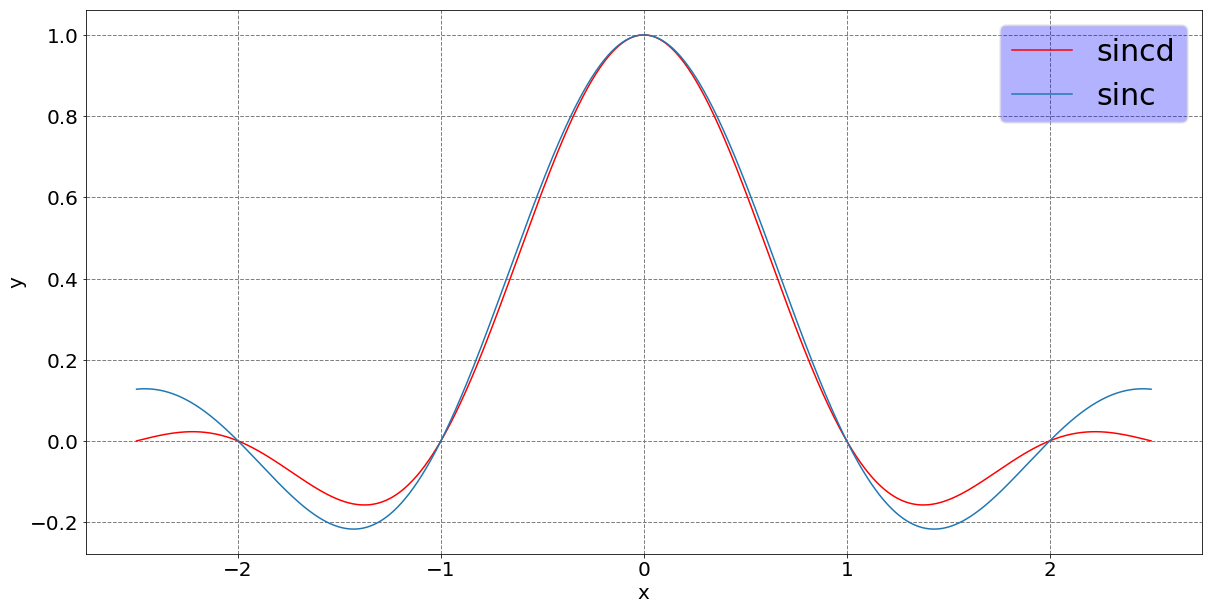
\includegraphics[height = 0.25\textheight]{6_5}
		\subcaption{Pour \(N = 5\)}
		\label{fig_6_5}
	\end{subfigure}
	\begin{subfigure}[b]{\textwidth}
		\centering
		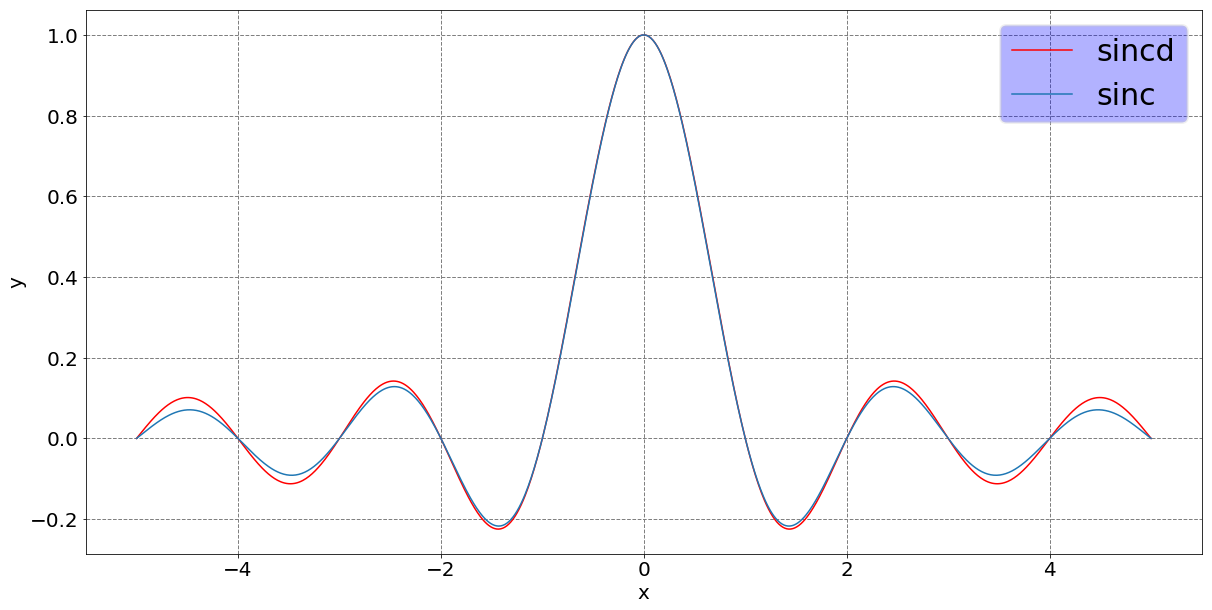
\includegraphics[height = 0.25\textheight]{6_10}
		\subcaption{Pour \(N = 10\)}
		\label{fig_6_10}
	\end{subfigure}
	\begin{subfigure}[b]{\textwidth}
		\centering
		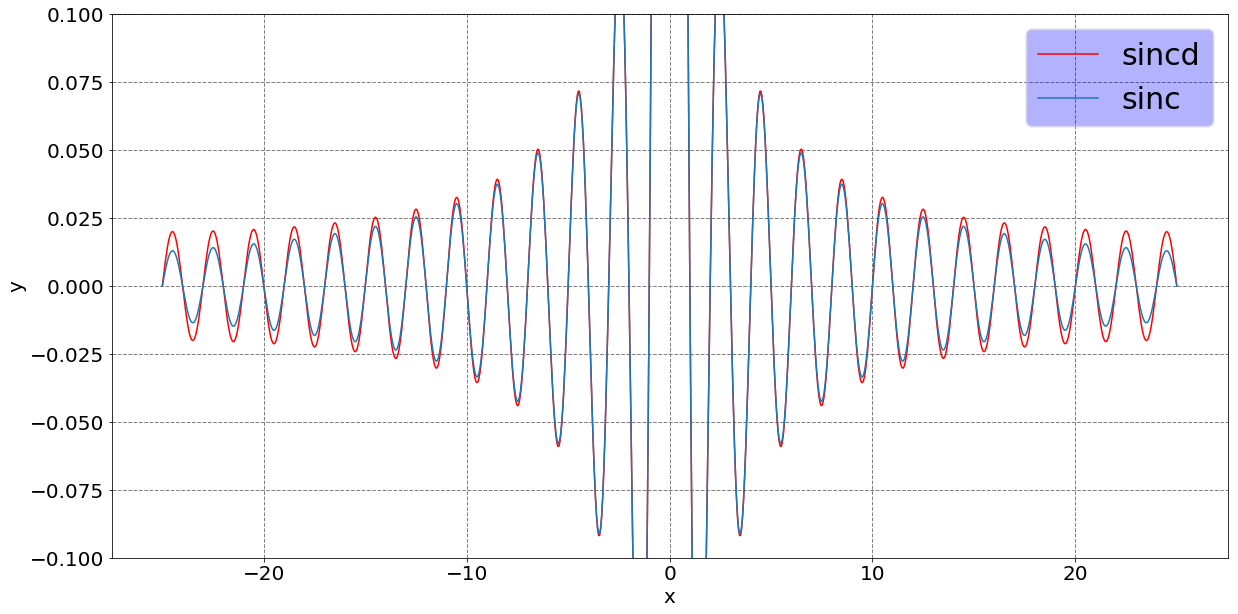
\includegraphics[height = 0.25\textheight]{6_50}
		\subcaption{Pour \(N = 50\)}
		\label{fig_6_50}
	\end{subfigure}
	\caption{Représentation graphique de la convergence du \(sincd_N\) et du \(sinc\), sur \([-N/2, N/2]\)}
	\label{fig_6}
\end{figure}

En figure~\ref{fig_6} sont représentés le \(sinc\) et le \(sincd_N\), pour différentes valeurs de \(N\) pour \(x \in[-N/2, N/2]\). On constate que, pour chaque valeur entière, on a bien égalité, et que, pour N assez grand, les différences sont minimes.

\section{Exercice 7}

\begin{figure}[H]
	\centering
	\begin{subfigure}[b]{\textwidth}
		\centering
		\begin{lstlisting}[frame = none, numbers = none]
		u = double(imread('lena.pgm'));
		\end{lstlisting}
		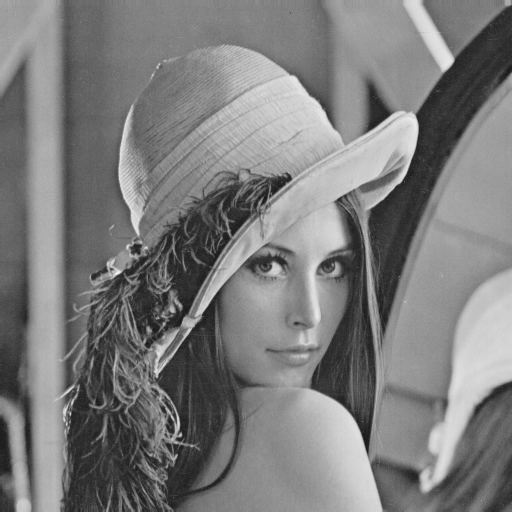
\includegraphics[scale = 1, height = 0.3\textheight]{lena.png}
		\subcaption{Image lena}
	\end{subfigure}
	\vspace{2cm}
	\begin{subfigure}[b]{\textwidth}
		\centering
		\begin{lstlisting}[frame=none, numbers = none]
		f = fft2(u);
		imshow(f, 'InitialMagnification', 100);
		\end{lstlisting}
		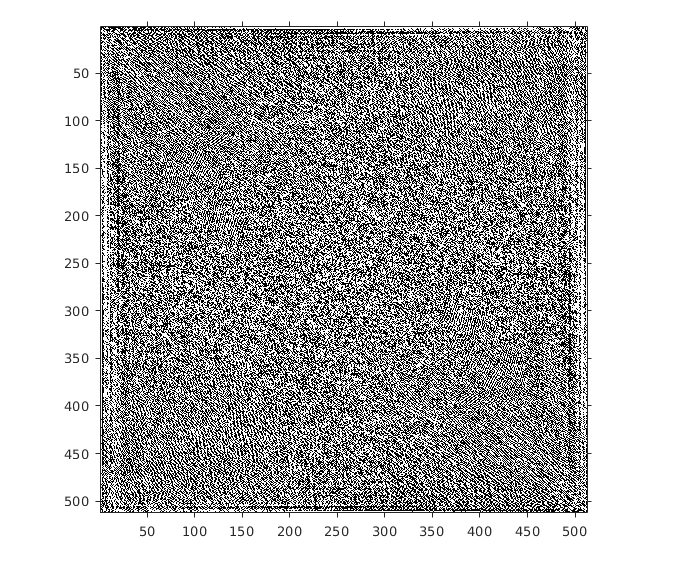
\includegraphics[scale = 1, height = 0.3\textheight]{7_1}
		\subcaption{Partie réelle de la transformée de Fourier de lena}
	\end{subfigure}
	\caption{Partie réelle de la transformée de Fourier de Lena}
	\label{7_1}
\end{figure}

En figure~\ref{7_1}, on demande à Matlab d'afficher en niveaux de gris une matrice complexe, résultant en un message d'erreur \textit{Warning: Displaying real part of complex input.}. On observe donc uniquement la partie réelle de la transformée de Fourier.

\begin{figure}[H]
	\centering
	\begin{subfigure}[b]{\textwidth}
		\centering
		\begin{lstlisting}[frame = none, numbers = none]
		imshow(abs(f));
		\end{lstlisting}
		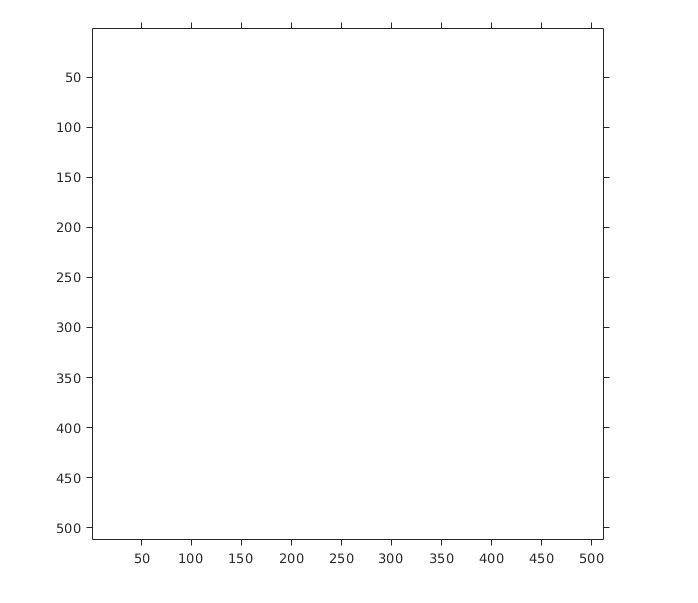
\includegraphics[scale = 1, height = 0.3\textheight]{7_21}
		\subcaption{Sans l'option [] de imshow}
		\label{7_21}
	\end{subfigure}
	\vspace{2cm}
	\begin{subfigure}[b]{\textwidth}
		\centering
		\begin{lstlisting}[frame=none, numbers = none]
		imshow(abs(f),[]);
		\end{lstlisting}
		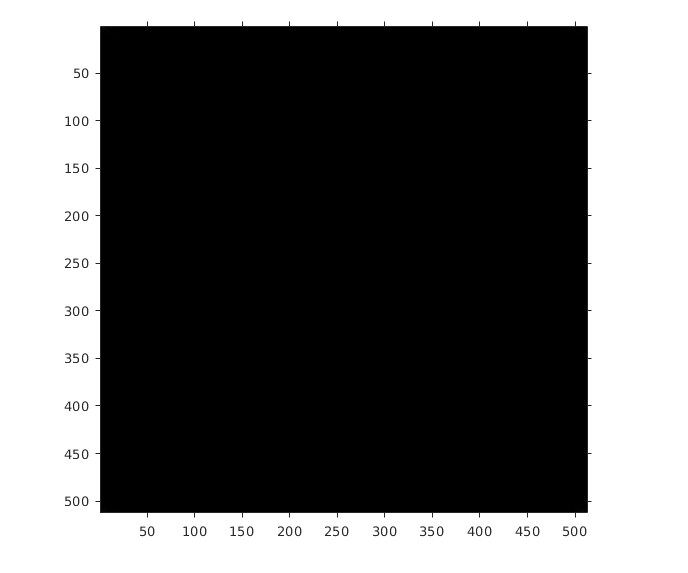
\includegraphics[scale = 1, height = 0.3\textheight]{7_22}
		\subcaption{Avec l'option [ ] de imshow}
		\label{7_22}
	\end{subfigure}
	\caption{Représentations du module de la transformée de Fourier}
	\label{7_2}
\end{figure}

En figure~\ref{7_2}, la commande~\ref{7_21} est équivalent à :
\begin{lstlisting}[numbers = none]
imshow(abs(f) > 1);
\end{lstlisting}
et on n'obtient que des pixels blancs, puisque imshow, quand on lui présente un double (ce qui est le type de abs(f)), représente en noir les valeurs à 0, en blanc les valeurs à 1, et en niveaux de gris les valeurs entre ces bornes. Or, on vérifie que abs(1) > 1 ne contient que des 1. En revance, avec l'option [ ], on rescale \(abs(f) \in [0, 1]\), avec la plus grande valeur en blanc, et la plus faible en noire. Or, la répartition des valeurs est très asymétrique, et on ne représente quasiment que du noir. On peut s'en convaincre en tracant le logarithme de cette image, qui donne la figure~\ref{7_33}.

\begin{figure}[H]
	\centering
	\begin{lstlisting}[frame=none, numbers = none]
	imshow(log(abs(f)),[]);
	\end{lstlisting}
	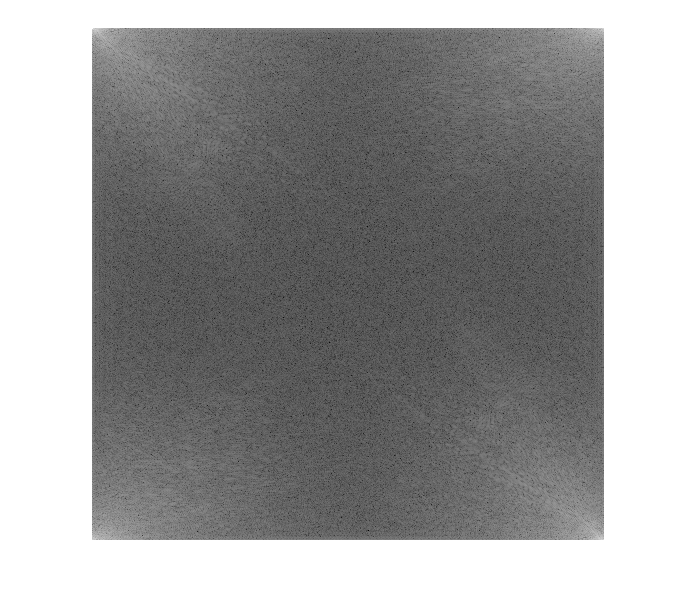
\includegraphics[height = 0.3\textheight]{7_33}
	\caption{Logarithme de la figure~\ref{7_22}}
	\label{7_33}
\end{figure}

En figure~\ref{7_3}, on sature \(1~\%\) des valeurs extremales du module de la transformée, et on redistribue linéairement les valeurs restantes sur tous les niveaux de gris. C'est ce que fait la fonction \textit{normsat}. La fonction \textit{fftshift} permet de centrer l'origine des fréquences, passant du coin supérieur gauche en figure~\ref{7_31} au centre en figure~\ref{7_32}.

\begin{figure}[H]
	\centering
	\begin{subfigure}[b]{\textwidth}
		\centering
		\begin{lstlisting}[frame = none, numbers = none]
		imshow(normsat(abs(f),1));
		\end{lstlisting}
		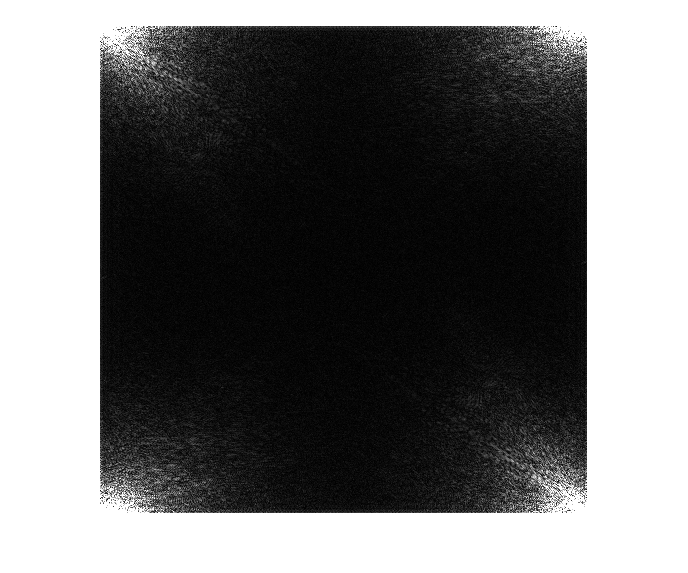
\includegraphics[scale = 1, height = 0.3\textheight]{7_31}
		\subcaption{Avec l'origine des fréquences en haut à gauche de l'image}
		\label{7_31}
	\end{subfigure}
	\vspace{2cm}
	\begin{subfigure}[b]{\textwidth}
		\centering
		\begin{lstlisting}[frame=none, numbers = none]
		imshow(normsat(fftshift(abs(f)),1));
		\end{lstlisting}
		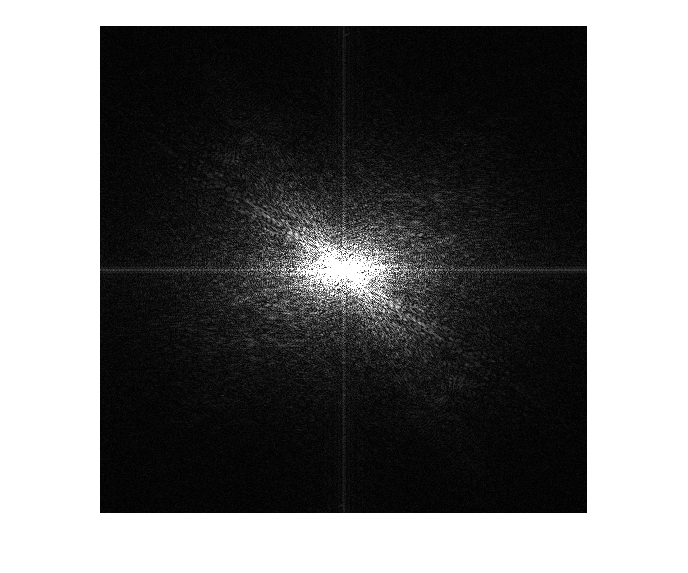
\includegraphics[scale = 1, height = 0.3\textheight]{7_32}
		\subcaption{Avec l'origine des fréquences au milieu de l'image}
		\label{7_32}
	\end{subfigure}
	\caption{Visualisation du module de la transformée de Fourier après saturation à \(1~\%\) des valeurs extremales et mapping linéaire des valeurs restantes en niveau de gris}
	\label{7_3}
\end{figure}

En figure~\ref{7_44} sont présentés les commandes et leur résultat pour visualier efficacement différentes parties d'une transformée de Fourier.

\begin{figure}
	\centering
	\begin{subfigure}[b]{0.45\textwidth}
		\centering
		\begin{lstlisting}[frame = none, numbers = none]
imshow(log(1 +abs(real(fftshift(f)))), [])
		\end{lstlisting}
		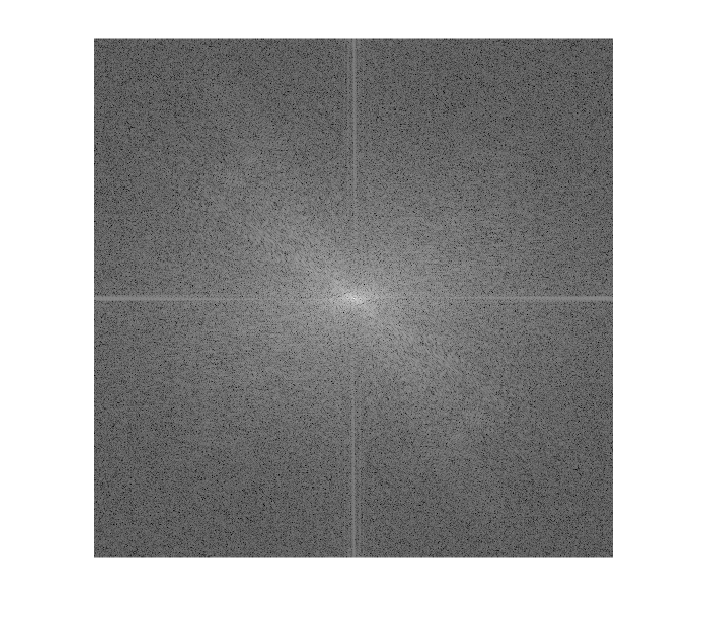
\includegraphics[scale = 1, width = \textwidth]{7_41}
		\subcaption{Logarithme de la partie réelle}
		\label{7_41}
	\end{subfigure}
	\begin{subfigure}[b]{0.45\textwidth}
		\centering
		\begin{lstlisting}[frame = none, numbers = none]
imshow(log(1 +abs(imag(fftshift(f)))), [])
		\end{lstlisting}
		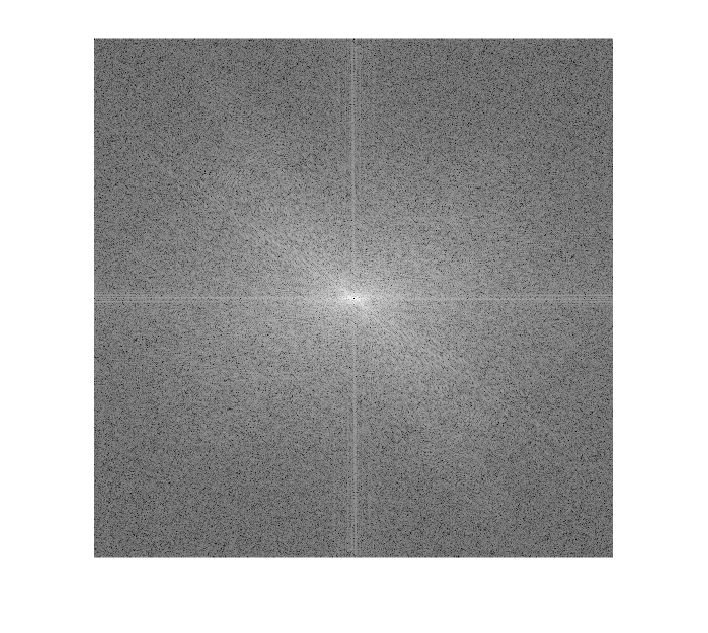
\includegraphics[scale = 1, width = \textwidth]{7_42}
		\subcaption{Logarithme de la partie imaginaire}
		\label{7_42}
	\end{subfigure}
	\begin{subfigure}[b]{0.45\textwidth}
		\centering
		\begin{lstlisting}[frame = none, numbers = none]
imshow(angle(fftshift(f)) + pi, [])
		\end{lstlisting}
		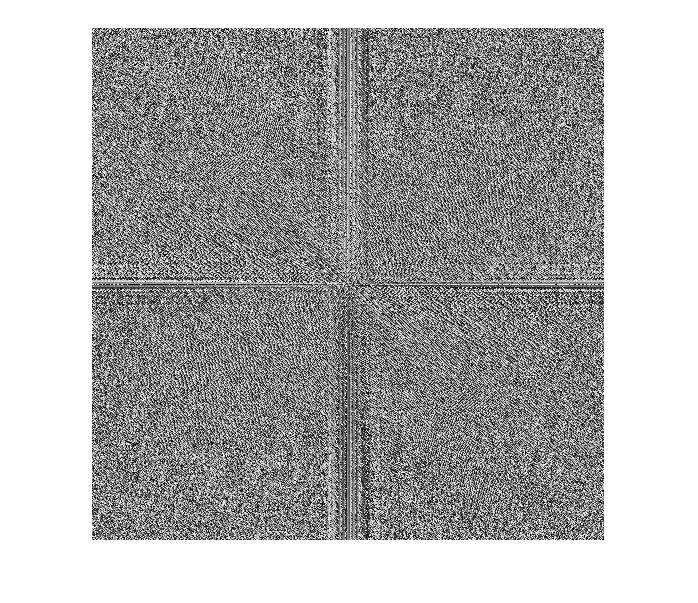
\includegraphics[scale = 1, width = \textwidth]{7_43}
		\subcaption{Phase}
		\label{7_43}
	\end{subfigure}
	\begin{subfigure}[b]{0.45\textwidth}
		\centering
		\begin{lstlisting}[frame = none, numbers = none]
imshow(log(1 +abs(fftshift(f))), [])
		\end{lstlisting}
		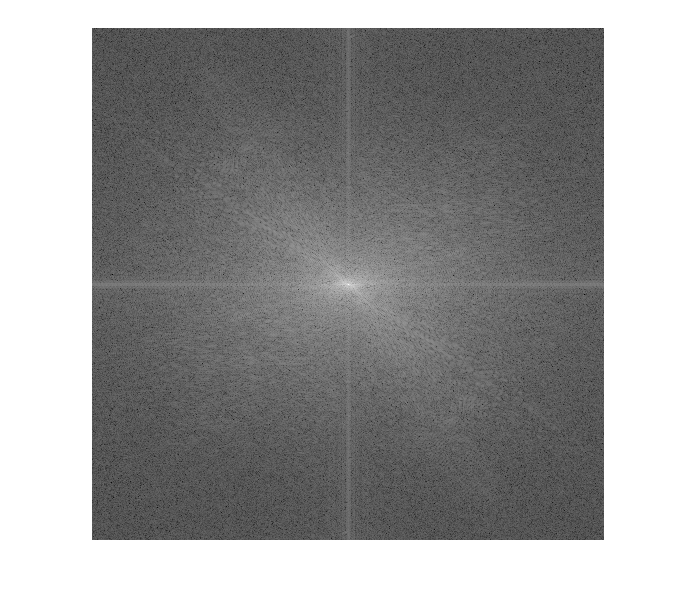
\includegraphics[scale = 1, width = \textwidth]{7_44}
		\subcaption{Logarithme du module}
		\label{7_44}
	\end{subfigure}
	\caption{Visualisation des divers parties d'une transformée de Fourier}
	\label{}
\end{figure}

\clearpage

\section{Exercice 8}


\end{document}
